\documentclass{article}
\usepackage{fullpage}

\usepackage{amsmath,cancel}
\usepackage{graphicx}
\usepackage{color}
\usepackage{alltt}
\newcommand{\red}[1]{{\color{red}#1}}
\newcommand{\cyan}[1]{{\color{cyan}#1}}
\newcommand{\blue}[1]{{\color{blue}#1}}
\newcommand{\magenta}[1]{{\color{magenta}#1}}
\newcommand{\yellow}[1]{{\color{yellow}#1}}
\newcommand{\green}[1]{{\color{green}#1}}
 
\newcommand{\bkt}[1]{\langle \mbox{ #1 } \rangle}
\newcommand{\br}{\mbox{~}|\mbox{~}}
 
\newcommand{\ns}[1]{\newpage {\bf #1}}

\setlength{\parindent}{0in}
 
\begin{document}
 
\huge

{\bf Big O definition}

\begin{align*}
  O(g(n)) &= \{ f(n) : &\mbox{there exists positive constants $c$ and $n_0$}\\
          &&\mbox{such that $0 \leq f(n) \leq cg(n)$ for all $n \geq n_0$}\}
\end{align*}
When we say
\begin{align*}
  f(n) &= O(g(n))
\end{align*}
we really mean
\begin{align*}
  f(n) &\in O(g(n))
\end{align*}
For example
\begin{align*}
  n^2 + 3n + 7 &= O(n^2)
\end{align*}
means
\begin{align*}
  f(n) &=  n^2 + 3n + 7
\end{align*}
is in the set
\begin{align*}
  O(n^2)
\end{align*}

\ns{$n^2 + 42n + 7 = O(n^2)$}

$n^2 + 42n + 7 \leq 2n^2$ for all $n \geq 50$

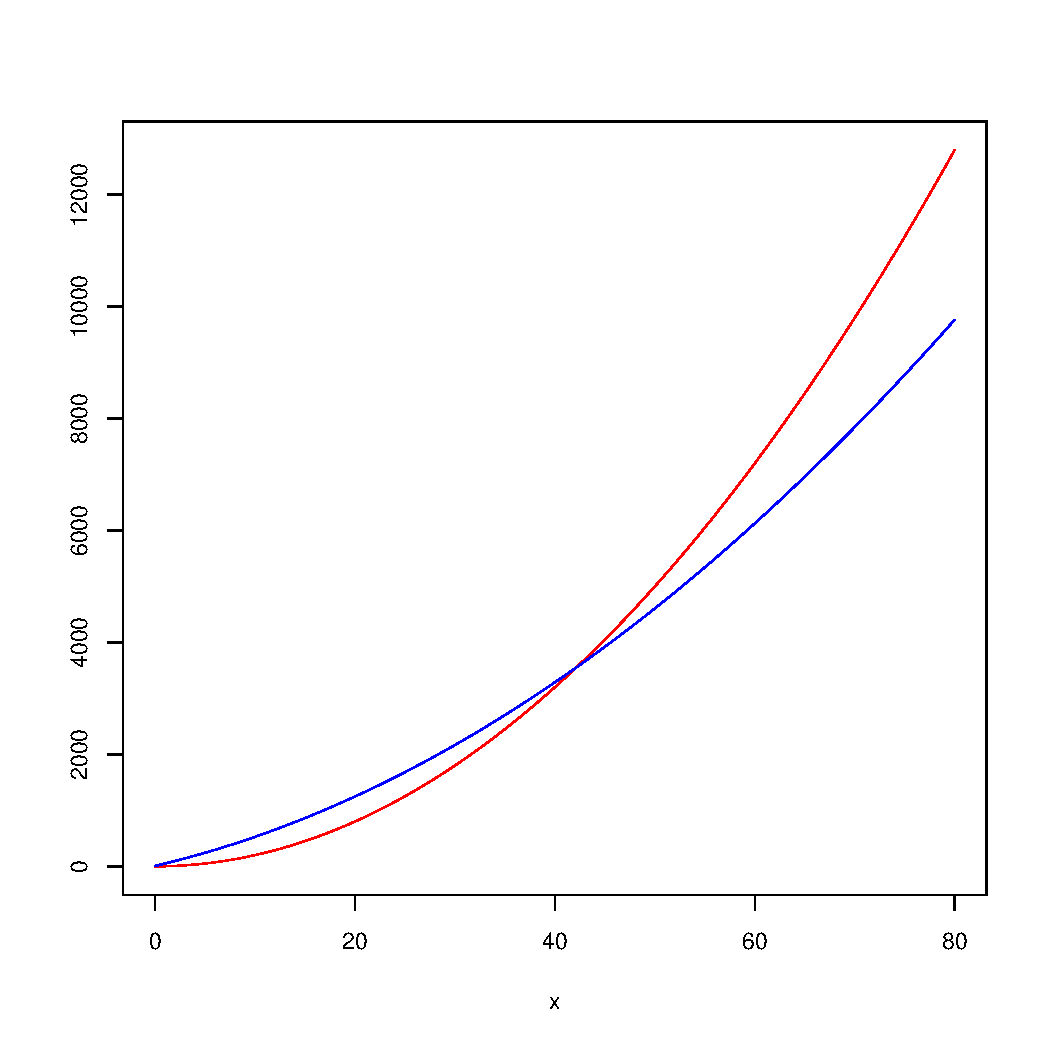
\includegraphics[width=\textwidth]{plot.pdf}


\ns{Proof of $n^2 + 42n + 7 = O(n^2)$}

\begin{align*}
  n^2 + 42n + 7 &\leq n^2 + 42n^2 + 7n^2 & \mbox{for $n \geq 1$}
  \\
  &= 50n^2
\end{align*}
So
$n^2 + 42n + 7 = O(n^2)$, with $c=50$ and $n_0 = 1$

\ns{Proof of $4n^2 + 5 n + 3 = O(n^2)$}
\begin{align*}
  4n^2 + 5 n + 3 &\leq   4n^2 + 5 n^2 + 3n^2 & n \geq 1\\
  &=  12n^2
  \end{align*}
so
$4n^2 + 5 n + 3 = O(n^2)$ with $c = 12$ and $n_0 = 1$

\ns{Proof of $5n\lg n + 8n - 200 = O(n\lg n)$}

Note: if $n\geq 2$ then $\lg n \geq 1$.

\begin{align*}
  5n\lg n + 8n - 200 &\leq 5n\lg n + 8n\\
  &\leq 5n\lg n + 8n \lg n & \mbox{for $n\geq 2$}\\
  &\leq 13 n\lg n
\end{align*}
So
\[
5n\lg n + 8n - 200 = O(n\lg n)
\]
with $c=13$ and $n_0=2$

\ns{Proof of $(n+5)\lg(3n^2+7) = O(n\lg n)$}
\begin{align*}
  (n+5)\lg(3n^2+7) &\leq (n+5n)\lg(3n^2 + 7n^2) & n \geq 1\\
  &=6n\lg(10n^2)\\
  &\leq 6n\lg(n^3) & n \geq 10\\
  &=6n(3\lg(n))\\
  &=18n\lg(n)
\end{align*}
So
$(n+5)\lg(3n^2+7) = O(n\lg n)$ for $c=18$ and $n_0=10$


\ns{Proof of $(n^2 + 5\lg n)/(2n+1) = O(n)$}

\begin{align*}
  \frac{n^2 + 5\lg n}{2n+1} &\leq \frac{n^2 + 5n^2}{2n +1} & n \geq 1\\
  &\leq \frac{n^2 + 5n^2}{2n } \\
  &= 3n
  \end{align*}
So
$(n^2 + 5\lg n)/(2n+1) = O(n)$ for $c=3$ and $n_0=1$


\ns{Useful facts}
\begin{itemize}
  \item For any $a < b$:
\[O(n^a) \subset O(n^b)\]

\item For any $a,b > 0, c > 1$:
  \[
  O(a) \subset O(\lg n) \subset O(n^b) \subset O(c^n)
  \]
  You can multiply to find
  \[
  O(an) = O(n) \subset O(n\lg n) \subset O(n^{b+1}) \subset O(nc^n)
  \]

\end{itemize}

\ns{Other sets}

\begin{align*}
  o(g(n))
  &=\\
  \{ f(n) : & \mbox{ for any positive constant $c$}\\
    &\mbox{there exists positive $n_0$ such that}\\
  &\mbox{$0 \leq f(n) < cg(n)$ for all $n \geq n_0$}\}\\
  O(g(n))
  &=\\
  \{ f(n) : & \mbox{ there exist positive constants $c$ and $n_0$ such that}\\
  &\mbox{$0 \leq f(n) \leq cg(n)$ for all $n \geq n_0$}\}\\
  \Theta(g(n))
  &=\\
  \{ f(n) : & \mbox{ there exist positive constants $c,d$ and $n_0$ such that}\\
  &\mbox{$0 \leq cg(n) \leq f(n) \leq dg(n)$ for all $n \geq n_0$}\}\\
  \Omega(g(n))
  &=\\
  \{ f(n) : & \mbox{ there exist positive constants $c$ and $n_0$ such that}\\
  &\mbox{$0  \leq cg(n) \leq f(n)$ for all $n \geq n_0$}\}\\
  \omega(g(n))
  &=\\
  \{ f(n) : & \mbox{ for any positive constant $c$}\\
    &\mbox{there exists positive $n_0$ such that}\\
  &\mbox{$0 \leq cg(n) < f(n)$ for all $n \geq n_0$}\}\\
\end{align*}

\ns{Number of anonymous functions}


The number of anonymous functions is equal to the number of times the
asymptotic notation appears.

\[\sum_{i=1}^{n} O(i) \]

Here we assume there is only one function, not $n$ different functions.


\ns{Asymptotic notation in equations}
\begin{description}
  \item[Right hand side:]
\[
2n^2 + 3n + 1 = 2n^2 + \Theta(n)
\]
means
\[
2n^2 + 3n + 1 = 2n^2 + f(n)
\]
for {\em some} $f(n)\in\Theta(n)$.
  \item[Left hand side:]
\[
2n^2 + \Theta(n) = \Theta(n^2)
\]
means for {\em all} $f(n)\in\Theta(n)$, 
\[
2n^2 + f(n) = \Theta(n^2)
\]
\item[We can chain them:]
  \begin{align*}
2n^2 + 3n + 1 &= 2n^2 + \Theta(n)\\
     &= \Theta(n^2)
  \end{align*}
  
\end{description}


\ns{Relational properties}
\begin{description}
\item[Reflexive:]
  \[
  f(n) = \Theta(f(n))
  \]
\item[Symmetric:]
  \[
  f(n) =\Theta(g(n)) \Leftrightarrow g(n) =\Theta(f(n))
\]
\item[Transitive:]
  \[
  (f(n) = \Theta(g(n))\ \wedge\ g(n) = \Theta(h(n))) \Rightarrow f(n) = \Theta(h(n))
  \]
\item[Transpose symmetry:]
  \[
  f(n) = O(g(n))\ \Leftrightarrow\ g(n) = \Omega(f(n))
  \]
  \[
  f(n) = o(g(n))\ \Leftrightarrow\ g(n) = \omega(f(n))
  \]

  \bigskip
\item
  Note:  We may have two functions $f$ and $g$ such that
  \begin{align*}
    f(n) &\not= o(g(n))\\
    f(n) &\not= O(g(n))\\
    f(n) &\not= \Theta(g(n))\\
    f(n) &\not= \Omega(g(n))\\
    f(n) &\not= \omega(g(n))
    \end{align*}
\end{description}

For example, $n^{1+\sin(n)}$ and $n$.

\ns{Limits}

\begin{align*}
  \lim_{n\rightarrow\infty} \frac{f(n)}{g(n)} = 0
  &\Longrightarrow
  f(n) = o(g(n))
  \\\\
  \lim_{n\rightarrow\infty} \frac{f(n)}{g(n)} = \infty
  &\Longrightarrow
  f(n) = \omega(g(n))
  \\\\
  \lim_{n\rightarrow\infty} \frac{f(n)}{g(n)} < \infty
  &\Longrightarrow
  f(n) = O(g(n))
  \\\\
  \lim_{n\rightarrow\infty} \frac{f(n)}{g(n)} > 0
  &\Longrightarrow
  f(n) = \Omega(g(n))
  \\\\
  \lim_{n\rightarrow\infty} \frac{f(n)}{g(n)} \in (0,\infty)
  &\Longrightarrow
  f(n) = \Theta(g(n))
\end{align*}

\ns{L'Hospital's Rule}

When
\begin{align*}
  \lim_{x\rightarrow\infty} f(x) &= \infty\\
  \mbox{and}\\
  \lim_{x\rightarrow\infty} g(x) &= \infty\\
\end{align*}
then
\begin{align*}
  \lim_{x\rightarrow\infty} \frac{f(x)}{g(x)} &= 
  \lim_{x\rightarrow\infty} \frac{f'(x)}{g'(x)}
\end{align*}

\end{document}





